\documentclass[11pt]{article}
\usepackage[pdftex]{graphicx, color}
\usepackage{listings}

\usepackage{tikz}
\usetikzlibrary{automata,positioning}

\headheight 8pt \headsep 20pt \footskip 30pt
\textheight 9in \textwidth 6.5in
\oddsidemargin 0in \evensidemargin 0in
\topmargin -.35in


\lstset{basicstyle=\small\ttfamily,breaklines=true}

\begin{document}
\begin{center}
% Change this:
\LARGE YOURNAME - SUNETID \\
\LARGE CS143 Spring 2021 - Written Assignment 1 \\
\end{center}

\begin{enumerate}
% problem 1
\item Write regular expressions for the following languages over the alphabet $\Sigma = \{0, 1\}$.  Hint some of these languages may include $\epsilon$.
\begin{enumerate}
    \item The set of all strings which do not end with $11$.
    \[
        % Answer Here
    \]
    \item The set of all strings representing a binary number where the sum of its bits is odd.
    \[
        % Answer Here
    \]
    \item The set of all strings where all characters are repeated at least once where ever they appear in the string (e.g. 00 or 000111100 but not 00100).
    \[
        % Answer Here
    \]
\end{enumerate}

\newpage

% problem 2
\item Draw DFA's for each of the languages from question 1. Note that a DFA must have a transition defined for every state and symbol pair. You must take this fact into account for your transformations. Your DFAs should not have more than 10 states.

\begin{enumerate}
    \item The set of all strings which do not end with $11$ \\
        % Answer Here
        % See piazza for tips on generating FSMs in latex or follow from the examples below
    \item The set of all strings representing a binary number where the sum of its bits is odd. \\
        % Answer Here
    \item The set of all strings where all characters are repeated at least once where ever they appear in the string (e.g. 00 or 000111100 but not 00100). \\
        % Answer Here
\end{enumerate}

\newpage

 % Problem 3
\item Using the techniques covered in class, transform the following NFAs over the alphabet $\{a, b, c\}$ into DFAs. Your DFAs should not have more than 10 states.  Note that a DFA must have a transition defined for every state and symbol pair, whereas a NFA need not. You must take this fact into account for your transformations. Hint: Is there a subset of states the NFA transitions to when fed a symbol for which the set of current states has no explicit transition?

Also include a mapping from each state of your DFA to the corresponding states of the original NFA.  Specifically, a state $s$ of your DFA maps to the set of states $Q$ of the NFA such that an input string stops at $s$ in the DFA if and only if it stops at one of the states in $Q$ in the NFA.

Tip: for readability, states in the DFA may be labeled according to the set of states they represent in the NFA.  For example, state $q_{012}$ in the DFA would correspond to the set of states $\{q_0, q_1, q_2\}$ in the NFA, whereas state $q_{13}$ would correspond to set of states $\{q_1, q_3\}$ in the NFA.


\begin{enumerate}
    \item Original NFA:\\
    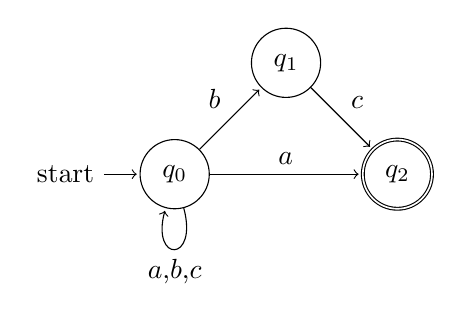
\begin{tikzpicture}[shorten >=1pt,node distance=2cm,on grid,auto]
        \node[state,initial] (q_0)   {$q_0$};
        \node[state] (q_1) [above right of=q_0] {$q_1$};
        \node[state,accepting] (q_2) [below right of=q_1] {$q_2$};
        \path[->]
        (q_0) edge [loop below] node {$a$,$b$,$c$} (q_0)
              edge  node  {$a$} (q_2)
              edge  node  {$b$} (q_1)
        (q_1) edge  node  {$c$} (q_2);
    \end{tikzpicture}
    \\
    DFA: \\
    % Answer Here
    \\
    Correspondences (DFA to NFA):
    \begin{itemize}
        \item % Answer Here
    \end{itemize}

    \item Original NFA: \\
    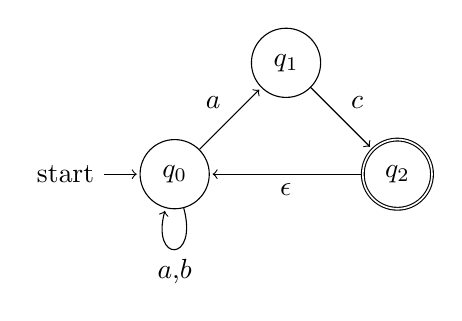
\begin{tikzpicture}[shorten >=1pt,node distance=2cm,on grid,auto]
        \node[state,initial] (q_0)   {$q_0$};
        \node[state] (q_1) [above right of=q_0] {$q_1$};
        \node[state,accepting](q_2) [below right of=q_1] {$q_2$};
        \path[->]
        (q_0) edge [loop below] node {$a$,$b$} (q_0)
              edge node {$a$} (q_1)
        (q_1) edge node {$c$} (q_2)
        (q_2) edge node {$\epsilon$} (q_0);
    \end{tikzpicture}
    \\
    DFA: \\
    % Answer Here
    \\
    Correspondences (DFA to NFA):
    \begin{itemize}
        \item % Answer Here
    \end{itemize}

    \item Original NFA:\\
    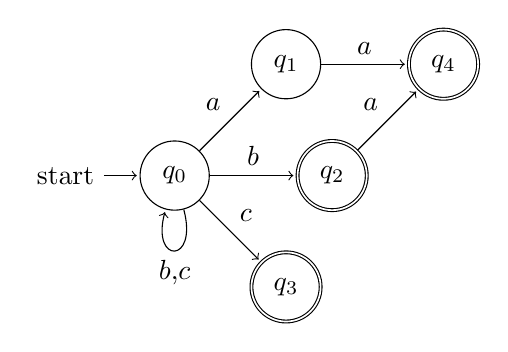
\begin{tikzpicture}[shorten >=1pt,node distance=2cm,on grid,auto]
        \node[state,initial] (q_0)   {$q_0$};
        \node[state] (q_1) [above right of=q_0] {$q_1$};
        \node[state,accepting] (q_2) [right of=q_0] {$q_2$};
        \node[state,accepting] (q_3) [below right of=q_0] {$q_3$};
        \node[state,accepting] (q_4) [right of=q_1] {$q_4$};
        \path[->]
        (q_0) edge [loop below] node {$b$,$c$} (q_0)
              edge node {$a$} (q_1)
              edge node {$b$} (q_2)
              edge node {$c$} (q_3)
        (q_1) edge node {$a$} (q_4)
        (q_2) edge node {$a$} (q_4);
    \end{tikzpicture}
    \\
    DFA: \\
    % Answer Here
    \\
    Correspondences (DFA to NFA):
    \begin{itemize}
        \item % Answer Here
    \end{itemize}
\end{enumerate}

\newpage

% Problem 4
\item Let $L$ be a language over $\Sigma = \{a, b, c\}$ where the following holds:

String $w$ is in $L$ if and only if $w$ is of the form $w = x^ns$ where $|x| = 1$, $n \geq 0$, and $s$ is a string that does not contain $x$ as a substring.  Here, $x^n$ denotes $x$ being repeated $n$ times.  You can imagine $w$ as a string with a head consisting of a character repeated 0 or more times and said character does not appears in the tail of $w$.

Examples of strings in $L$: \underline{c}abab, \underline{bbb}, \underline{bb}aaac, baab

Examples of strings \textbf{not} in $L$: \underline{b}aaa\underline{b}c, \underline{c}ab\underline{c}ab

Draw an NFA for $L$.  Your solution should not have more than 10 states.

NFA:
% Answer Here

\newpage

% Problem 5
\item Consider the following tokens and their associated regular expressions, given as a \textbf{flex} scanner specification:

\begin{lstlisting}
%%
(01|10)                   printf("apple");
1(01)*0                   printf("banana");
(1011*0|0100*1)           printf("coconut");
\end{lstlisting}

Give an input to this scanner such that the output string is $\tt (apple^{\rm 3}  banana)^{\rm 3}(apple\ coconut)^{\rm 2}$, where $\tt A^i$ denotes {\tt A} repeated {\tt i} times.   (And, of course, the parentheses are not part of the output.)  You may use similar shorthand notation in your answer.

\[
    % Answer Here
\]


\newpage

% Problem 6
\item Recall from the lecture that, when using regular expressions to scan an input, we resolve conflicts by taking the largest possible match at any point. That is, if we have the following \textbf{flex} scanner specification:

\begin{lstlisting}
%%
do                      { return T_Do; }
[A-Za-z_][A-Za-z0-9_]*  { return T_Identifier; }
\end{lstlisting}

and we see the input string ``dot'', we will match the second rule and emit T\_Identifier for the whole string, not T\_Do.

However, it is possible to have a set of regular expressions for which we can tokenize a particular string, but for which taking the largest possible match will fail to break the input into tokens. Give an example of a set of regular expressions and an input string such that: a) the string can be broken into substrings, where each substring matches one of the regular expressions, b) our usual lexer algorithm, taking the largest match at every step, will fail to break the string in a way in which each piece matches one of the regular expressions. Explain how the string can be tokenized and why taking the largest match won't work in this case.


\textbf{Answer:} % Answer Here

\end{enumerate}
\end{document}